In this section, we outline the application of the \brfcs\ tool towards the development of a UAV surveillance system.
The motivation was to showcase the utility and capability of the BriefCASE toolchain on an industrial scale problem, to determine whether the technology provides designers with early validation of their model; produces early information about cyber-vulnerabilities; provides effective mitigations; and handles a complex real-world message format, namely  the UxAS message format.

%apply the BriefCASE tool towards the development of a UAV surveillance system in which
In this surveillance system, the UAV receives commands from a ground station to conduct surveillance over a geographical region. In response, the UAV's on-board mission computer generates a flight plan consisting of a series of waypoints that the UAV must traverse to complete its mission. The UAV is also given a set of \textit{keep-in} and \textit{keep-out} zones that may constrain its flight path.

We have modeled the system architecture of the UAV in AADL.  The model includes a Mission Computer for communicating with the ground station and generating flight plans, and a Flight Control Computer for UAV navigation.  The Mission Computer architecture model includes hardware components such as a processor, memory, and communication devices, as well as software.
%
The initial software architecture model (shown in \figref{fig:sw-initial}) contains drivers for communication with the Ground Station and Flight Control Computer, a Waypoint Manager component that provides flight plan coordinates to the Flight Control Computer, and the Flight Planner.  The Flight Planner is the open-source UxAS software developed by AFRL~\cite{uxas}.

For this application, UxAS accepts three types of messages.  The \textit{Operating Region} message defines where the UAV can and cannot fly.  The \textit{Line Search Task} message contains a series of waypoints that the UAV should traverse.  The waypoints typically lie along some geographical feature of interest, such as a river or railway.  Note that the UAV may not be able to directly traverse the Line Search Task waypoints due to no-fly zone constraints specified in the Operating Region message.  Anytime after receiving the Operating Region and Line Search Task messages, a Ground Station can transmit an \textit{Automation Request} message, which instructs UxAS to generate a flight plan that satisfies these constraints.  UxAS passes the flight plan in an \textit{Automation Response} message to the Waypoint Manager.  Because the Flight Control Computer can only process a small number of waypoints at a time, the Waypoint Manager parcels a small number of waypoints corresponding to the current UAV position, and sends them to the Flight Control Computer over a serial connection via the UART Driver.

\begin{figure*}[h]
	\centering
	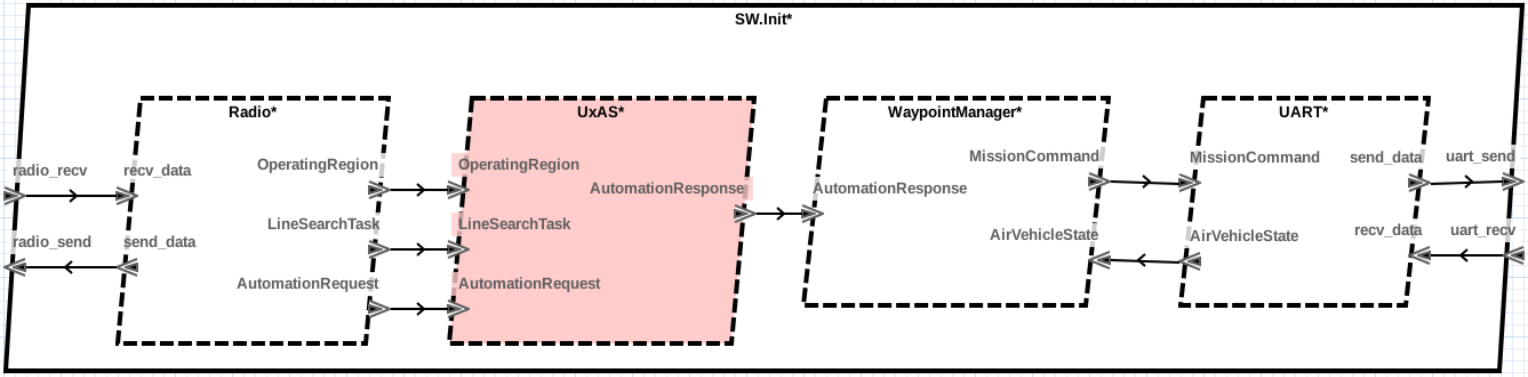
\includegraphics[width=2\columnwidth]{figs/sw-initial.png}
	\caption{Initial software architecture.}
	\label{fig:sw-initial}
\end{figure*}

Within the software model, we have formalized some of the high-level requirements as assume-guarantee contracts.  We perform a formal analysis with \agr\ to verify that the model satisfies the contracts.  For the initial version of our design, the verification passes.
%
Although we are satisfied with the results of the formal verification using AGREE, we have not yet analyzed the design for cyber-vulnerabilities.

In \brfcs, we analyze the model using one (or more) of the integrated cybersecurity analysis tools.
As the designers of the system, we reviewed the list of potential vulnerabilities, and then added new requirements to the system model.
%  To satisfy these requirements we need to mitigate the vulnerabilities discovered by the analysis by modifying the design.
%
For example, the vulnerbility analysis noted that UxAS is an open source project, so we marked that component as \texttt{uncontroled} (colored red in \figref{fig:sw-initial}) and added requirements for ensuring that unverified or malicious code (which could potentially be embedded in the component) is not able impact other components.

In total, we added seven cyber requirements from the vulnerability analysis into our model.  These include four wellformedness requirements on data, two requirements for monitoring the behavior of the open-source UxAS component, and an attestation requirement for ensuring the Ground Station software has not been tampered with.  Requirements are imported into the model as goals in the assurance case.  Because we can build the assurance case at any time during development, we can easily determine for a given snapshot of the model which requirements are not yet supported by evidence.

The intent of the wellformedness requirements is to prevent
malformed messages from causing a buffer overrun or code injection
attack.  In the UAV design, such messages are most likely to originate
from a remote source or the uncontrolled UxAS component.  By placing
filters on the connections upstream of mission-critical components,
such attacks could be mitigated.  The Filter transform is therefore
applied for each wellformedness requirement, inserting filter
components on the incoming and outgoing UxAS connections.

The filter code contracts for the four UxAS connections are similar, and check that record values contained in the messages are within appropriate ranges.  For example, the Automation Response message filter, which drops messages containing malformed flight plans, is defined as shown in \figref{fig:automation-response-filter}.  Although \texttt{Latitude}, \texttt{Longitude} and \texttt{Altitude} are defined as 64-bit floating-point values, the filter only passes messages containing waypoint values between [-90,90], [-180,180], and [0,15000], respectively.

\begin{figure}[h]
	\centering
	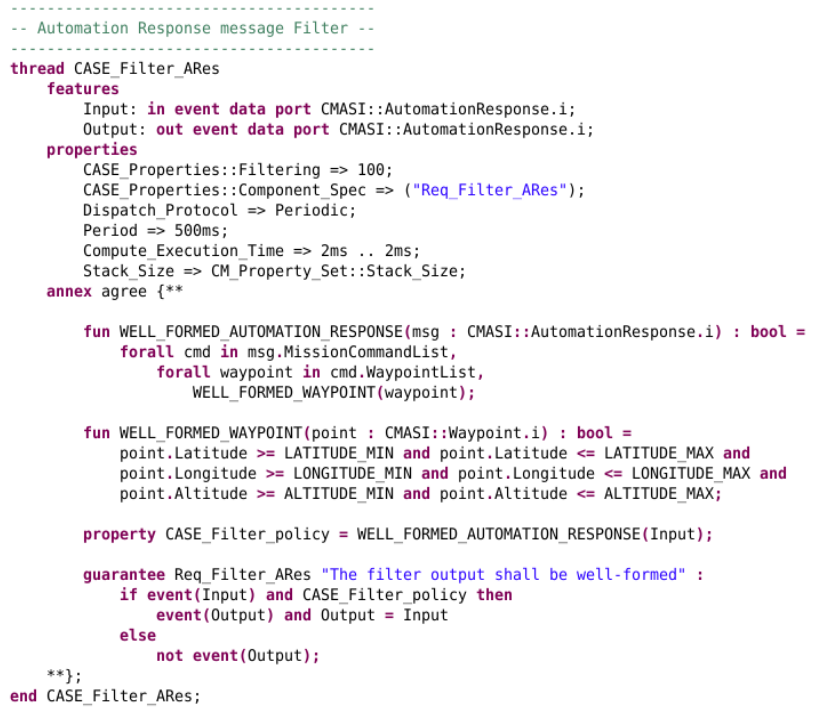
\includegraphics[width=1\columnwidth]{figs/automation-response-filter.png}
	\caption{Automation Response Filter specification.}
	\label{fig:automation-response-filter}
\end{figure}

In addition to monitoring the UxAS output for malformed messages, we must also monitor for suspicious behavior.  This requires adding components for detecting that UxAS has crashed, as well as monitoring the correctness of the flight plans it produces.  The Monitor transform is applied for this class of mitigation.  We add a \textit{response} monitor to send an alert if UxAS does not emit a response within a set amount of time from receiving a request.  And we add a \textit{geofence} monitor to ensure that generated flight plans are compliant with the specified keep-in and keep-out zones.  The Geofence Monitor is a gated monitor in that it prevents the observed automation response from reaching the Waypoint Manager if the zones are violated.
The Geofence Monitor code contract is shown in \figref{fig:geofence-monitor}.

% \begin{figure}[h]
% 	\centering
% 	\includegraphics[width=1\columnwidth]{figs/response-monitor.png}
% 	\caption{Response Monitor specification.}
% 	\label{fig:response-monitor}
% \end{figure}

\begin{figure}[h]
	\centering
	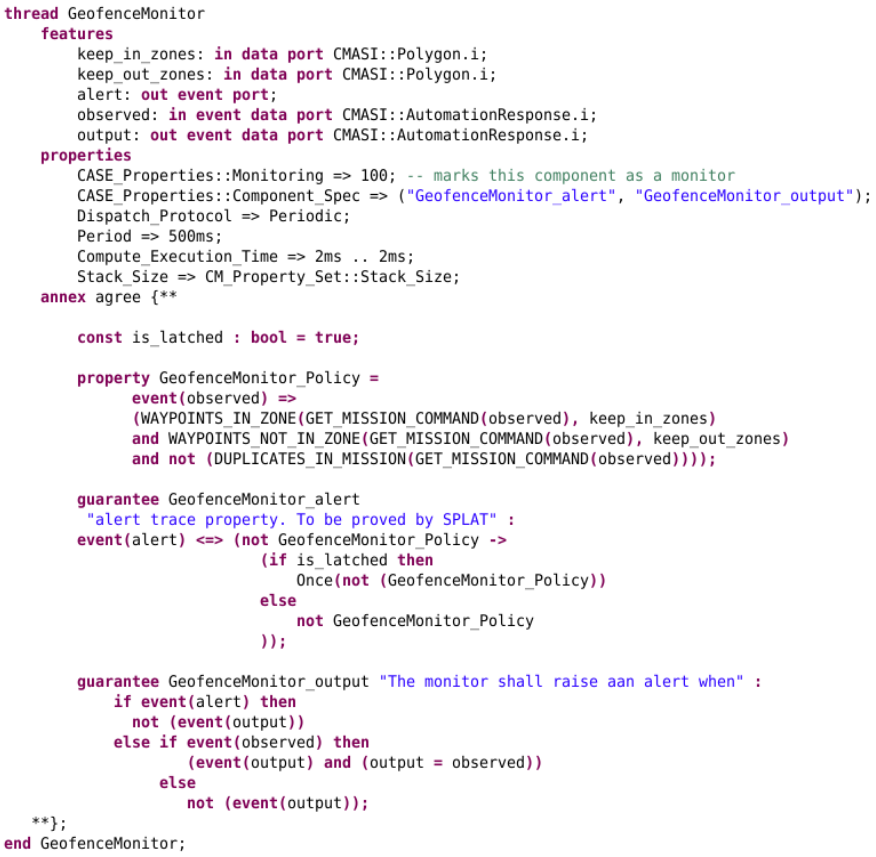
\includegraphics[width=1\columnwidth]{figs/geofence-monitor.png}
	\caption{Geofence Monitor specification.}
	\label{fig:geofence-monitor}
\end{figure}

So far, we have addressed requirements that
%The requirements that have been addressed so far
mitigate vulnerabilities related to malformed messages and malicious behavior \textit{on-board} the UAV.  But we also want to protect against a compromised ground station transmitting well-formed, but malicious, commands. The final cyber requirement is mitigated by a transform that adds two components to the UAV software: an Attestation Manager for evaluating remote systems like the Ground Station, and an Attestation Gate for filtering messages from sources that have not been approved by the Attestation Manager.  The Attestation Manager \ckml\ implementation is automatically inserted into the application code base by \brfcs. The code contract for the Attestation Gate is completely generated by the transform since its behavior is specific to attestation.

After transforming the model to address the cyber requirements, the software architecture now appears as shown in \figref{fig:hardened-sw}.  The shaded components (green) were added by the transform with the exception of the UxAS component (red). 

After unit testing the monitors, we formally verify the model with \agr\ to show that all of the component contracts are satisfied.
We then run \splt\ to produce provably-correct code.
The synthesized code is output to a directory in the build file system with the location specified for each component in the model.  The corresponding correctness proof is used in our assurance case as additional evidence that the vulnerability has been properly mitigated.

\begin{figure*}[h]
	\centering
	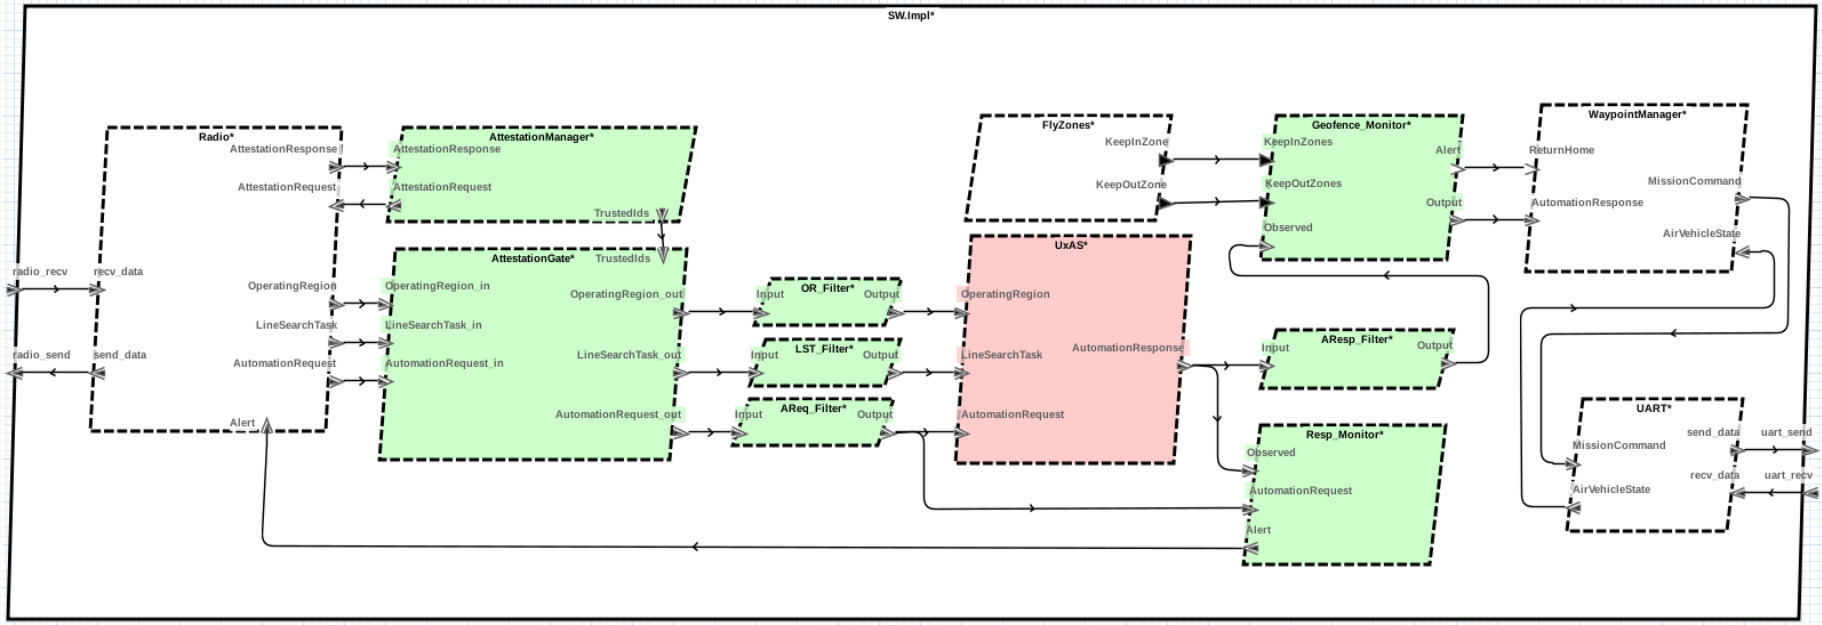
\includegraphics[width=2\columnwidth]{figs/hardened-sw.png}
	\caption{Cyber-resilient software architecture.}
	\label{fig:hardened-sw}
\end{figure*}

Once we have determined that the model is correct and satisfies its cyber requirements, and the software components in the model have been implemented, either by \splt\ or other means, the system can be built and deployed.  We run the HAMR tool to generate the component stubs and infrastructure code necessary to enable component communication and execution according to a specified schedule.
% HAMR translates the AADL system model to code that implements threading infrastructure and inter-component communication consistent with the AADL computational model.
%
HAMR then compiles the software to execute on seL4.

The UAV and Ground Station software were deployed on ODROID XU4 hardware, and communicated with each other over ethernet.  The AMASE flight simulator, representing the Flight Control Computer was run on a Linux machine and connected to the UAV ODROID via a serial connection.  The UxAS implementation on the UAV was modified by adding malicious code that would prevent it from responding to Automation Requests or produce flight plans that would violate the operating region constraints.  Some of the Line Search Task messages transmitted from the Ground Station contained malformed messages that would modify the UxAS behavior. In addition, we modified the Ground Station to simulate a breach for our evaluation of the attestation transform.
%
We performed a set of tests on the initial system (\figref{fig:sw-initial}) prior to applying our cyber-resiliency mitigations in order to verify the effectiveness of the malicious code.
A third party evaluator repeated the tests on the hardened system and % were able to
demonstrated that our mitigation strategy was successful.
%The following scenarios were exercised (status messages from the high-assurance components in the hardened system are in \figref{fig:mitigation-output}):
The following scenarios were exercised:

\paragraph{Infected Ground Station} An application file is modified on the Ground Station, which sends the UAV on a mission-violating trajectory.
On the hardened system, messages sent to the UAV were rejected by the Attestation Manager.

\paragraph{Malformed Line Search Task message} The Line Search Task message contained a waypoint with a longitude outside the permitted range to exploit vulnerabilities in the on-board software.  The wellformedness filter for Line Search Task messages prevented this message from reaching the UxAS.

\paragraph{UxAS vulnerability exploit} Line Search Tasks with greater than 90 waypoints were transmitted from the Ground Station, triggering a vulnerability that crashes UxAS.   When this occurs, UxAS is unable to generate an Automation Response. The response monitor detected and signaled the Ground Station when UxAS failed to respond to the request.

\paragraph{UxAS trojan modifies flight plan} A trojan embedded in UxAS attempts to cause the UAV to fly into a specified keep-out zone by modifying the mission command waypoints in the Automation Response.
On the hardened system the Geofence Monitor detected that it was being instructed to fly into a keep-out zone and returned the UAV to Home Base.

\subsection{Discussion}

\newjunk{
The case study demonstrated the viability of writing code contracts and synthesizing implementations from code contracts in a real-world system. It additionally provided insights for improvement.  We discovered very early that we needed a mechanism to test contracts.  We initially used the synthesis path with a custom test harness for the synthesized code, but this proved to be slow and cumbersome because we had to move back and forth between the OSATE environment and an external test platform. Test contracts are a direct result of our experience, and they obviate the back and forth by integrating test into the modeling and analysis environment.
}

\newjunk{
Writing code contracts for the more complex monitors revealed that although the language is very effective at declarative specifications that define what is being calculated, it is non-intuitive, and sometimes cumbersome, for defining how the computation needs to take place. The primary reason for its unease in describing how computation is performed is that it lacks any type of iterative looping structure for arrays. Instead, it relies on folding and mapping to describe iterative computation which is non-intuitive for many types of array updates. Growing the expressiveness of the language arround arrays is something to investigate in future work.
}


\newjunk{
	There are several, practical, low-level concerns that need to be addressed in the high-level model before synthesis takes place that in our process were only discovered after running the actual system on the designated hardware and software. We specifically found it difficult to know the memory bounds for heaps, stacks, and buffers and time bounds for the scheduler \emph{a priori} to code synthesis. As a result, we would have to employ a costly iterative approach to set bounds, synthesize code, and then check if anything failed. Integrating better memory and running time analysis at the modeling level is something to investigate in future work.  
}
% \begin{figure}[h]
% 	\centering
% 	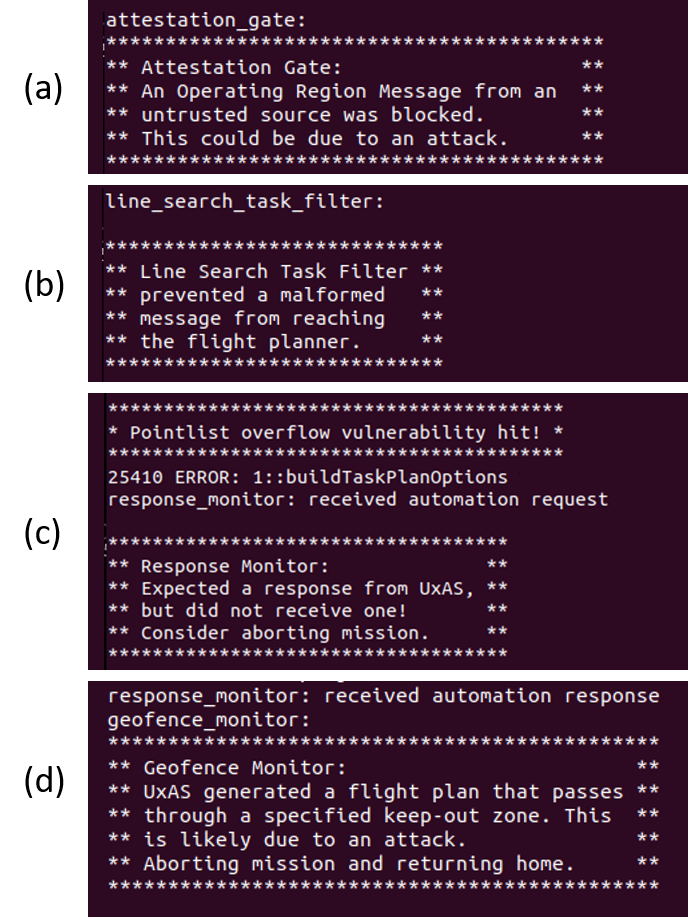
\includegraphics[width=0.8\columnwidth]{figs/mitigation-output.png}
% 	\caption{Cyber-resilient system response.}
% 	\label{fig:mitigation-output}
% \end{figure}
